%-------------------------------------------------------------------------------
\chapter{Speciális platformok megjelenése}
%-------------------------------------------------------------------------------
\section{hybrid deep learning}
%TODO Nincs befejezve

\section{nGraph}
A most leírtak alapját az nGraph hivatalos dokumentációja adja\cite{web:ngraph_intro}.
Az nGraph az Intel\registeredlogo által fejlesztett programkönyvtár és egy futtatási környezet/fordító készlet melyet mély tanuló projektekhez.
Legszembetűnőbb tulajdonsága, hogy képes többféle hardver architektúrán futtatni és beépíthető számos keretrendszerbe.
Ezek azok a jellemzők, amiket kerestünk témavezetőmmel, hogy mély tanulást tudjunk végeztetni hatékonyan a \emph{HuSSar-on}. 
Ezen túlmenően a jövőbeli fejlesztések az iparban egyre jelentősebben igényelik, hogy a modern MI rendszerek skálázhatóak legyenek, mert egyrészt a neurális hálók egyre komplexebbé válnak, másrészt az általuk feldolgozott adatok mennyisége is rohamosan növekszik.

Jelenleg két bevett gyakorlat van a mély tanulás felgyorsítására:
\begin{enumerate}
	\item \textbf{Dedikált hardver tervezése a mély tanulással kapcsolatos számításokhoz} -- Sok vállalkozás tervez \emph{Alkalmazásspecifikus integrált áramköröket} (ASIC) neurális hálózatok betanítására és futtatására.
	\item \textbf{Szoftver optimalizáció} -- Programkönyvtárakat tartalmazó fejlesztési keretrendszerek fejlesztése, melyek képesek a hálózatokkal kapcsolatos számításokat több szálon, optimalizáltan futtatni. Az nGraph, mint fordító is egy ilyen megoldás.
\end{enumerate}

\subsection{Motiváció}
A mai legmodernebb szoftveres megoldás mély tanulásra az, ha integrálunk kernel könyvtárakat\footnote{Programkönyvtár, mely neurális hálókkal kapcsolatos elemi, \emph{mag} függvényeket tartalmazzák} mély tanulási keretrendszerekbe.
Ilyen integráció lehet például ha a Tensorflow keretrendszer alatt az Nvidia CuDNN könyvtárát használjuk.
A {kernel könyvtárak} egy adott célarchitektúrára optimalizált kernelekből és egyéb műveleti szintű optimalizálásokból állnak, ezekkel érve el teljesítménynövekedést.
Azonban a kernel könyvtáraknak három fő problémája van:
\begin{enumerate}
	\item Nem biztosítanak gráf szintű optimalizálást
	\item A keretrendszerek integrációja a {kernel könyvtárakkal} nem skálázható
	\item A szükséges lefordított kernel könyvtárak száma növekszik, ahogy új processzorok jelennek meg
\end{enumerate}
Az nGraph fordító megoldás az első két problémára, és a \emph{PlaidML}-el ötvözve kiküszöbölhető a harmadik probléma.
\subsection{Gráf szintű optimalizálás}
Az nGraph dokumentációjában áll egy példa arra vonatkozóan, hogyan lehet, hogy egy mély tanulási keretrendszer integrálva egy {kernel könyvtárral} a számításokat optimálisan végzi, mégis a számítási gráf a csúcsait alkotó műveletek szempontjából mégsem optimális.
\begin{figure}[!ht]
	\centering
	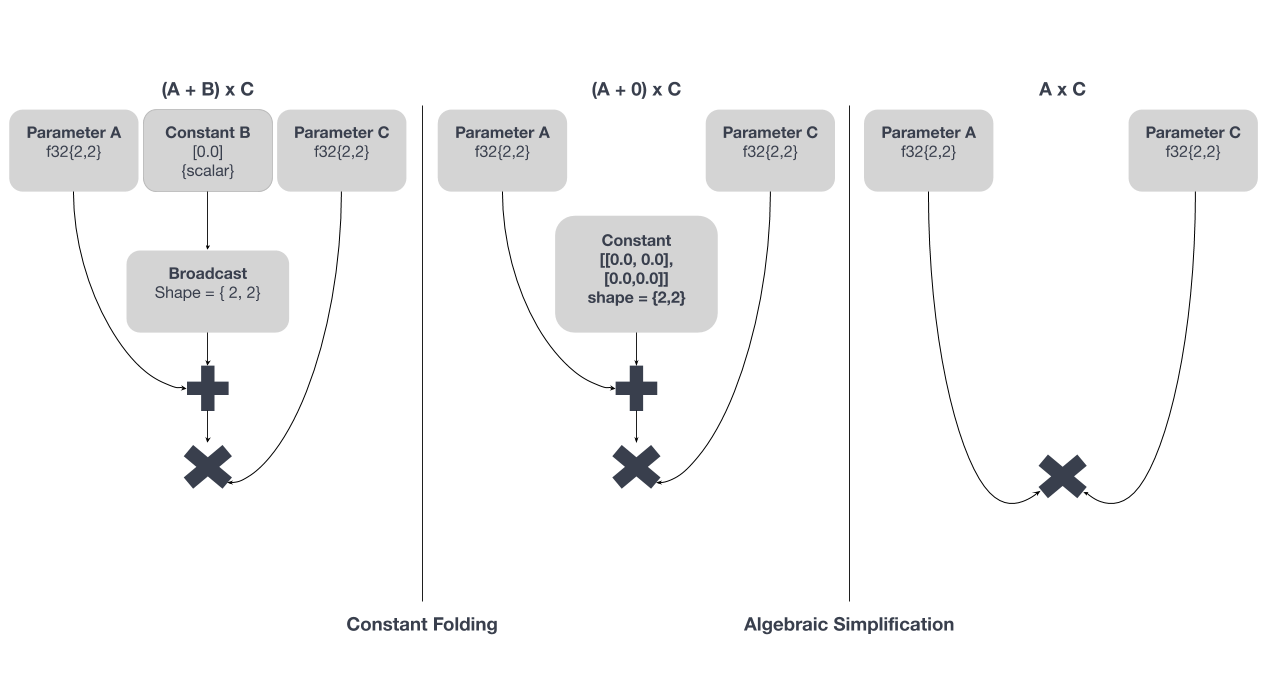
\includegraphics[width=0.9\textwidth]{kernel-problem-1.png}
	\caption{két optimalizálás módszer: konstans összehajtás és algebrai egyszerűsítés a gráfon. \protect \footnotemark}
	\label{fig:grafoptimalizalas}
\end{figure}
\footnotetext{forrás: \cite{web:ngraph_intro}}
A fenti ábra bemutatja, hogyan egyszerűsíthetünk az $A$,$B$ és $C$ tenzorokat feldolgozó, $ (A+B)*C $ tenzorműveletet végrehajtó számítási gráfon.
Fordítási időben megállapítható, hogy $B$ egy skalár konstans, így a \emph{konstans összehajtásnak} nevezett optimalizálás elvégezhető, és a 2 dimenziós vektorrá való kiterjesztés művelete elhagyható (helyette inkább közvetlenül létrehozunk egy $2\times2$ tenzort).
Ebben a példában $B=0$ skalár volt, így a belőle létrejött tenzor egy nullmátrix, így az semleges a kifejezés kiértékelésének szempontjából.
\emph{Algebrai egyszerűsítést} végezve az $ (A+0)*C $ leegyszerűsíthető az $A*C$ kifejezésre, így összesen két csúccsal csökkentettük a gráfunkat.
Ez az optimalizáció tehát a számítási gráf szintjén lett elvégezve.
Így belátható, hogy a mély tanulási keretrendszerbe integrált kernel programkönyvtárak nem optimális futást végeznek, hiába a műveletek szintjén elért optimalizálás. 
\subsection{Skálázható keretrendszer integráció}
Ahogy gyarapodik a mély tanuláshoz használható gyorsítókártya architektúrák és keretrendszerek száma, a meglévő mély tanulást alkalmazó fejlesztési platformok bővítése egyre több munkát igényel és egyre nő a hibák megjelenésének a valószínűsége. Az integráció kapható készen, szakértő fejlesztőcsapatoknak kell implementálnia.
Minden új keretrendszert manuálisan kell integrálni a meglévő hardverek kernel könyvtárával és minden újonnan megjelenő hardvercsalád meghajtó programkönyvtárát be kell integrálni egyesével a meglévő keretrendszerekbe.
Ez a munka önmagában is hatalmasra tud nőni, de egy sok eszközből álló összeállítás nagyon törékeny és költséges a fenntartása.
Az nGraph úgy oldja meg ezt a problémát, hogy ún. \emph{hidakat} alkalmaz, amikkel integrálható valamelyik mély tanulási keretrendszerbe.
A híd megkapja a keretrendszerben megalkotott számítási gráfot vagy ahhoz hasonló struktúrát és átalakítja egy ún. \emph{közbenső reprezentációvá}\footnote{IR: Intermediate Representation}. Ezzel kaptunk egy egységes, platformfüggetlen számítási gráfot, így nem kell egy új programkönyvtárat beintegrálni minden egyes meglévő keretrendszer alá, elegendő csak az, hogy az nGraph-ban, mint programkönyvtárban implementált \emph{primitív műveleteket} támogassa az új programkönyvtár.
\subsection{Növekvő kernel szám}
Egy kernel könyvtár integrálása egyszerre több mély tanulási keretrendszerrel nehéz feladat és egyre komplexebbé válik, ahogy növekszik az optimális teljesítményhez szükséges kernelek száma.
Régen a mély tanulással kapcsolatos kutatások egy kis számú \emph{primitív} számítást használtak, mint a konvolúció, általános mátrixszorzás, stb. Az MI kutatás előrehaladtával és az ipari mély tanuló alkalmazások továbbfejlesztésével, a szükséges kernelek száma (k) exponenciálisan nő.
Ez a szám a processzor architektúrák számán (h), adattípusokon (t), műveleteken (p) és az egyes paraméterek számosságán (p) alapul ($ k = h \times t \times m \times p $).
\begin{table}[!ht]
	\centering
	\begin{tabular}{|c|c|c|c|}
		
		Hardver & Művelet & Adattípus & Paraméterek \\ 
		\hline
		CPU & konvolúció & 16 bites lebegőpontos & NCHW vagy NHWC \\ 
		
		GPU & MatMul & 32 bites lebegőpontos & 2D, 3D és 4D tenzorok \\ 
		
		FPGA & Normalizálás & 8 bites egész &  \dots \\ 
		
		\dots & \dots & \dots & \\
	\end{tabular} 
	\caption{Néhány példa, tényezőnként hányféle esetre kell külön fordítani  kernelt könyvtárt }
	\label{table:kernels}
\end{table}

Ezen probléma megoldásához jön képbe a PlaidML. Ez egy \emph{tenzor fordító}\footnotemark, mely azt célozza, hogy képes legyen neurális hálózatokat tanítani és futtatni bármilyen típusú hardveren. Más szavakkal segíti a magas szintű keretrendszerek (Keras, ONNX, nGraph) integrálni olyan ezsközökkel, melyekhez nincs meg a szükséges támogatás vagy a meglévő szoftverkészlet hozzájuk szigorúan linceszelt.\cite{github:PlaidML}\cite{web:PlaidML}
\footnotetext{Olyan fordító, melynek nyelve arra lett fejlesztve, hogy főleg tenzorműveleteket igénylő számításokat tudjunk hatékonyan programozni}

Az nGraph tehát integrálható a PlaidML-el. Elsősorban az nGraph a platform független IR-rel igyekszik orvolsoni a skálázható backend-el kapcsolatos kihívást. A PlaidML ezt megtámogatja azzal, hogy képes az IR-ből származó gráfokból LLVM, OpenCL, OpenGL, CUDA és Metal kódot generálni melyek a megfelelő hardveren futtathatóak. Így egy magas szintű keretrendszerben írt neurális háló lefordul Intel és AMD processzrokon valamint grafikus processzorokon, az nVidia processzorain, továbbá az Apple cég által feljelsztett eszközökön.

Az nGraph gráf szintű optimalizációját ráadásul kiegészíti automatikusan a PlaidML alacsonyabb szinten, ezzel teljesítmény növekedést érve el.

Összegzésül tehát az nGraph feldarabolja a neurális hálózathoz tartozó számítási gráfot processzor architektúrának megfelelően, majd ezen gráfokat a PlaidML lefordítja a megfelelő kódokra, melyeket aztán a célprocesszorokra lefordítunk és futtatunk.

%TODO ide még jöhetne egy nGraph használatát bemutató alfejezet 
\section{Myriad X és az Intel Neural Computer Stick 2}
%Motiváció: Valós idejű alkalmazások esetén szükséges az offline számítás -> GPU - lehetséges, de erőforrás igényes(áram és hűtés) és nagy méretű 
Ma az iparban mély tanulással működő modern alkalmazások nagy méretű és teljesítményű számítógépeket igényelnek. Erre az igényre válaszul felhő szolgáltatást nyújtó vállalatok külön platformot építettek ki. Az ilyen kliens-szerver architektúrájú gépi tanulás hatékony lehet, azonban a valós-idejű alkalmazásoknál és hordozható eszközökben történő felhasználásnál komoly hátrányt jelenthet a hálózati késleltetés. Hogy ilyen területeken is alkalmazható legyen a mély tanulás, hardvergyártók olyan kis energiafogyasztású \emph{alkalmazás-specifikus integrált áramkörök} fejlesztésére törekedtek, melyek képesek neurális hálózatokat hatékonyan futtatni. Ilyen az Intel által kifejlesztett Myriad X lapka is, melyet főleg \emph{gépi látáshoz} terveztek.

Maga a Myriad egy Videójel feldolgozó processzor széria, melynek 3. generációja a Myriad X architektúrája kiegészült egy úgynevezett \emph{Neural Compute Engine-el}, mely a betanított hálózatok futtatását hivatott gyorsítani. Ezzel együtt a lapka 16 darab 128-bit VLIW processzormagok, ún. SHAVE magot és 2,5MB 400GB/s sávszélességű memóriát tartalmaz. Számításokat 8bites egészek és 16bites lebegőpontos váltózókon tud végezni.\footnote{forrás: https://www.movidius.com/myriadx} 
% TODO Myriad X

A Myriad X kifejlesztésén túlmenően a vállalat tervezett egy gyorsítókártyát is ehhez a processzorhoz, melyet Neural Compute Stick (NCS) névvel forgalmaz. Az Intel kiadta a második verzióját az eszköznek  Neural Compute Stick 2 (NCS2) névvel és az első verziót nem forgalmazz már. Ezért a továbbiakban a leírtakat az NCS2-re kell érteni.
Az eszköz USB 3.0 -ás interfésszel rendelkezik, így sok gazdagéppel használható, többek között Raspberry Pi-vel is. Meghajtására az Intel OpenVINO eszközkészlete használható, melyet gépi látáson alapuló alkalmazások fejlesztésére készített a vállalat. Lehetőség van egy platformon több NCS2 modul együttes használatára, így egyszerűen növelhető a rendszer teljesítménye.
\begin{figure}[h]
	\centering
	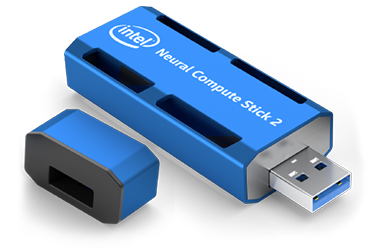
\includegraphics[width=0.5\linewidth]{fig/NCS2-specs}\\
	\footnotesize forrás:https://software.intel.com/en-us/neural-compute-stick
	\caption{Neural Compute Stick 2 gyorsító} 
	\label{fig:ncs2-specs}
\end{figure}
%TODO Nincs Befejezve

\subsection{Az NCS2 használata OpenVINO keretrendszerben}
Az alábbiak alapját az Intel OpenVINO eszközkészletének dokumentációja adja.\cite{web:OpenVINO} A dokumentációban a felépített neurális hálózatokra modell néven hivatkoznak, amit most én is átveszek.

Az OpenVINO eszközkészlet alkalmas arra, hogy gyorsan készítsünk olyan alkalmazásokat, melyek valamilyen módon emulálják az emberi látást. Képesek vagyunk segítségével az NCS2-n kívül más Intel gyártmányú hardverrel dolgozni, például Intel CPU-n és integrált GPU-n. Továbbá népszerű keretrendszereket támogat, mint a TensorFlow, Caffe, MXNet vagy az ONNX. Az eszközkészlet komponensekei közül az alábbiakat emelném ki:
\begin{description}[noitemsep]
	\item[Inference Engine] python API, aminek segítségével különböző gyorsítókártyák megszólíthatók egységes módon.
	\item[Model Optimizer] parancssoros alkalmazás mentett modellek átkonvertálására. Ahhoz, hogy a különböző keretrendszerekben megalkotott modelleket egységesen tudja kezelni az Inference Engine, szükség van azok átkonvertálására egy platformfüggetlen struktúrába.
	\item[OpenCV] az OpenCV közösségi fejlesztésű verziójának Intel hardverekre fordított változata.
\end{description}

Az OpenVINO-val való munka folyamatának három fő lépése van:
\begin{enumerate*}[label={}, font=\bfseries]
	\item Betanított Neurális hálózat beszerzése;
	\item a hálózat átkonvertálása a Model Optimizer-rel;
	\item python szkript implementálása az Inference Engine-t tartalmazó modulokkal, melyben az átkonvertált fájlokat lefuttatjuk a célhardveren
\end{enumerate*}

\section{Google Edge TPU}
Az Intelhez hasonlóan a Google is tervezett célprocesszort és hozzá fejlesztő panelt, mély tanulást alkalmazó projektekhez. A Google Edge TPU-ról és a Coral USB Accelerator-ról a Heartbeat internetes magazinban megjelent cikkben értesültem.\cite{web:GoogleEdge} A Google TPU-ról szerzett ismereteim a wikipédia ,,Tensor Processing unit'' cikkéből szereztem.\cite{wiki:TPU}

\begin{figure*}[h]
	\centering
	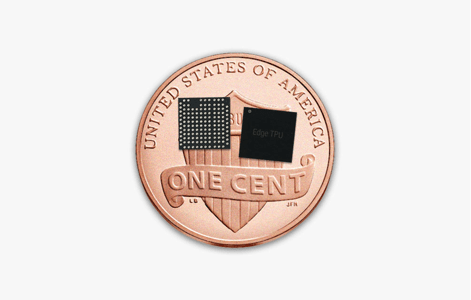
\includegraphics[width=0.4\textwidth]{fig/penny-edge-tpu}\\
	\footnotesize forrás: https://cloud.google.com/edge-tpu/
	\caption{Edge TPU}
	\label{fig:EdgeTPU}
\end{figure*}
\begin{figure*}[h]
	\centering
	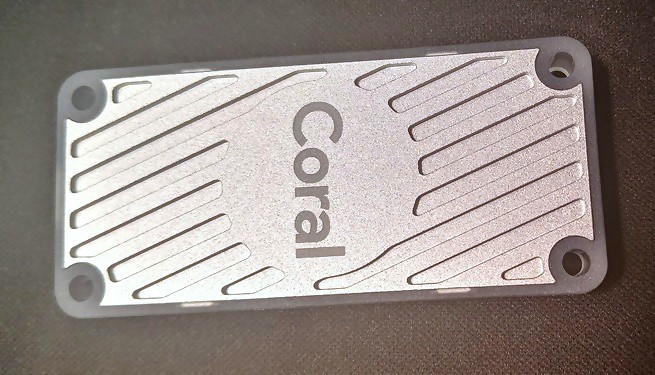
\includegraphics[width=0.4\textwidth]{fig/Coral_USBAccelerator}\quad
	\caption[Coral USB Accelerator]{Az Edge TPU-t építették az USB interfésszel ellátott Coral USB Accerlerator-ba.\cite{web:GoogleEdge}}
	\label{fig:coralusbaccelerator}
\end{figure*}


A Google a Tensor Processing Unit\texttrademark-ot, egy saját fejlesztésű alkalmazásspecifikus integrált áramkört használ a neurális hálózatokkal kapcsolatos számítások optimalizálására. Ezek lényegében mátrix műveletekre számítására fejlesztett processzorok CISC utasításkészlettel. Három generációt ért meg, az első még csak 8-bites egészeken tudott műveleteket végezni, azonban már a második generáció képes volt lebegőpontos számításokra is. A Tensor processing unit-okkal felszerelt gyorsítókártyákat a Google saját adatközpontjaiban használja főként és elérhetővé teszi őket a \emph{Google Cloud Platform} nevű szolgáltatásán keresztül. Nevéből adódóan a kártya architektúrája lehetővé teszi, hogy  tenzorműveletek tudjanak hatékonyan végrehajtani, utasításkészletük kifejezetten támogatja a neurális hálózatokat. Ilyen művelet a konvolúció és az \ref{sect:neuralNetworkTheory} alfejezetben tárgyalt aktváló függvények alkalmazása a mátrix szorzáson túl.

Az Edge TPU a cég szerverei által használt TPU-hoz viszonyítva kisebb méretben és energiafogyasztásban. Ugyan azt az igényt igyekszik kielégíteni, mint a korábban bemutatott Myriad X processzor. Azzal összehasonlítva viszont képes neurális hálózatok tanítására is korlátozott mértékben. Az Edge TPU részét képezi a Google Coral eszközkészletének, mellyel alternatívát nyújtanak a felhőalapú Cloud AI szolgáltatással szemben. A Coral különböző fajtájú hardvert nyújt a felhasználóknak, mindegyik központi eleme az Edge TPU. Az eszköz programozásához használható API-t az Edge TPU python könyvtár (\verb|edgetpu| python modul) valósítja meg, amely képes TensorFlow Lite-ban alkotott betanított neurális hálózatok futtatására. A könyvtár kulcsfontosságú interfészeit a következő osztályok képezik.Képosztályozási feladatokhoz a \verb|ClassificationEngine| használatos, vizuális objektumazonosításra a \verb|DetectionEngine|. Az \verb|ImprintingEngine| és \verb|SoftmaxRegression| az ún. \emph{transzfer tanuláshoz} alkalmazható, vagyis előre betanított hálózatok a feladatnak megfelelő újratanítását végezhetjük el vele.


\section{Új gyorsítók: Intel Nervana Neural Network Processor}

%TODO Nincs Befejezve